%----------------------------------------------------------------------------------------
%	PACKAGES AND THEMES
%----------------------------------------------------------------------------------------
\PassOptionsToPackage{table}{xcolor}
\documentclass[aspectratio=169,xcolor=dvipsnames,svgnames,x11names,fleqn]{beamer}
% \documentclass[aspectratio=169,xcolor=dvipsnames,fleqn]{beamer}

\usetheme{RedVelvet}

\usefonttheme[onlymath]{serif}



\usepackage{xspace}
\usepackage{amsmath}
\usepackage{amssymb}
\usepackage{amsfonts}
\usepackage{color}
\usepackage{physics}
% \usepackage{mathbb}
\usepackage{rahul_math}
\usepackage{bigints}

\usepackage{graphicx} % Allows including images
\usepackage{booktabs} % Allows the use of \toprule, \midrule and \bottomrule in tables
\usepackage{tikz,pgfplots}
\usepackage{subfigure}
\usetikzlibrary{arrows}
\usepackage{minted}
\definecolor{LightGray}{gray}{0.9}
\definecolor{cream}{rgb}{0.92, 0.9, 0.55}
\definecolor{lightblue}{rgb}{0.68, 0.85, 0.9}


\usepackage{xcolor-material}
\usetikzlibrary{fit}
\tikzset{%
apple/.pic={
  \fill [MaterialBrown] (-1/8,0)  arc (180:120:1 and 3/2) coordinate [pos=3/5] (@)-- ++(1/6,-1/7)  arc (120:180:5/4 and 3/2) -- cycle;
  \fill [MaterialLightGreen500] (0,-9/10)  .. controls ++(180:1/8) and ++(  0:1/4) .. (-1/3,  -1) .. controls ++(180:1/3) and ++(270:1/2) .. (  -1,   0) .. controls ++( 90:1/3) and ++(180:1/3) .. (-1/2, 3/4) .. controls ++(  0:1/8) and ++(135:1/8) .. (   0, 4/7)
}
}

\newcommand{\leftdoublequote}{\textcolor{blue}{\scalebox{3}{``}}}

\newcommand{\rightdoublequote}{\textcolor{blue}{\scalebox{3}{''}}}


\usepackage{textcomp}

\usepackage{overpic}

%----------------------------------------------------------------------------------------
%	TITLE PAGE
%----------------------------------------------------------------------------------------

\usepackage{tikz-qtree,tikz-qtree-compat}
\usetikzlibrary{calc}


\title[CPE 486/586: Machine Learning]{CPE 486/586: Machine Learning for Engineers} % The short title appears at the bottom of every slide, the full title is only on the title page
\subtitle{02 Tools for Machine Learning}

\author[Rahul Bhadani] {{\Large \textbf{Rahul Bhadani}}}

\institute[UAH] % Your institution as it will appear on the bottom of every slide, maybe shorthand to save space
{
    Electrical \& Computer Engineering,  The University of Alabama in Huntsville
}
\date

% \titlegraphic{
%    \includegraphics[width=0.4\linewidth]{figures/UAH_primary.png}
% }

\begin{document}

%-------------------------------------------------
\begin{frame}
    \titlepage
\end{frame}

%-------------------------------------------------
\begin{frame}{Outline}
    \backgroundtableofcontents
\end{frame}


\section{Command Line Tools and Linux}

\begin{frame}
    \sectionpage
\end{frame}

\begin{frame}{Why Command Line Tools and Linux}

\begin{enumerate}
    \item Download data from another location, webpage or server \begin{center}
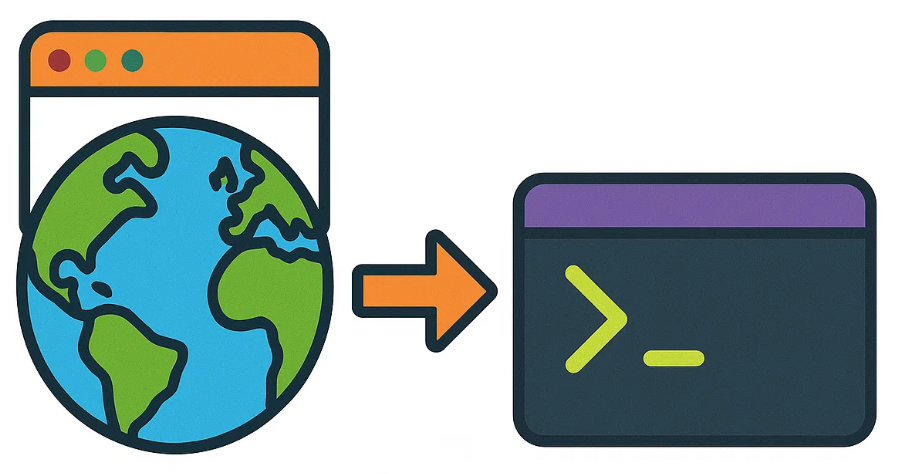
\includegraphics[height=.4\textheight]{figures/cmd_line_download.png}
\end{center}
\end{enumerate}
    
\end{frame}

\begin{frame}{Why Command Line Tools and Linux}

\begin{enumerate}
    \setcounter{enumi}{1}
    \item File operation, renaming, copying, editing, etc, in bulk. 
    \begin{center}
        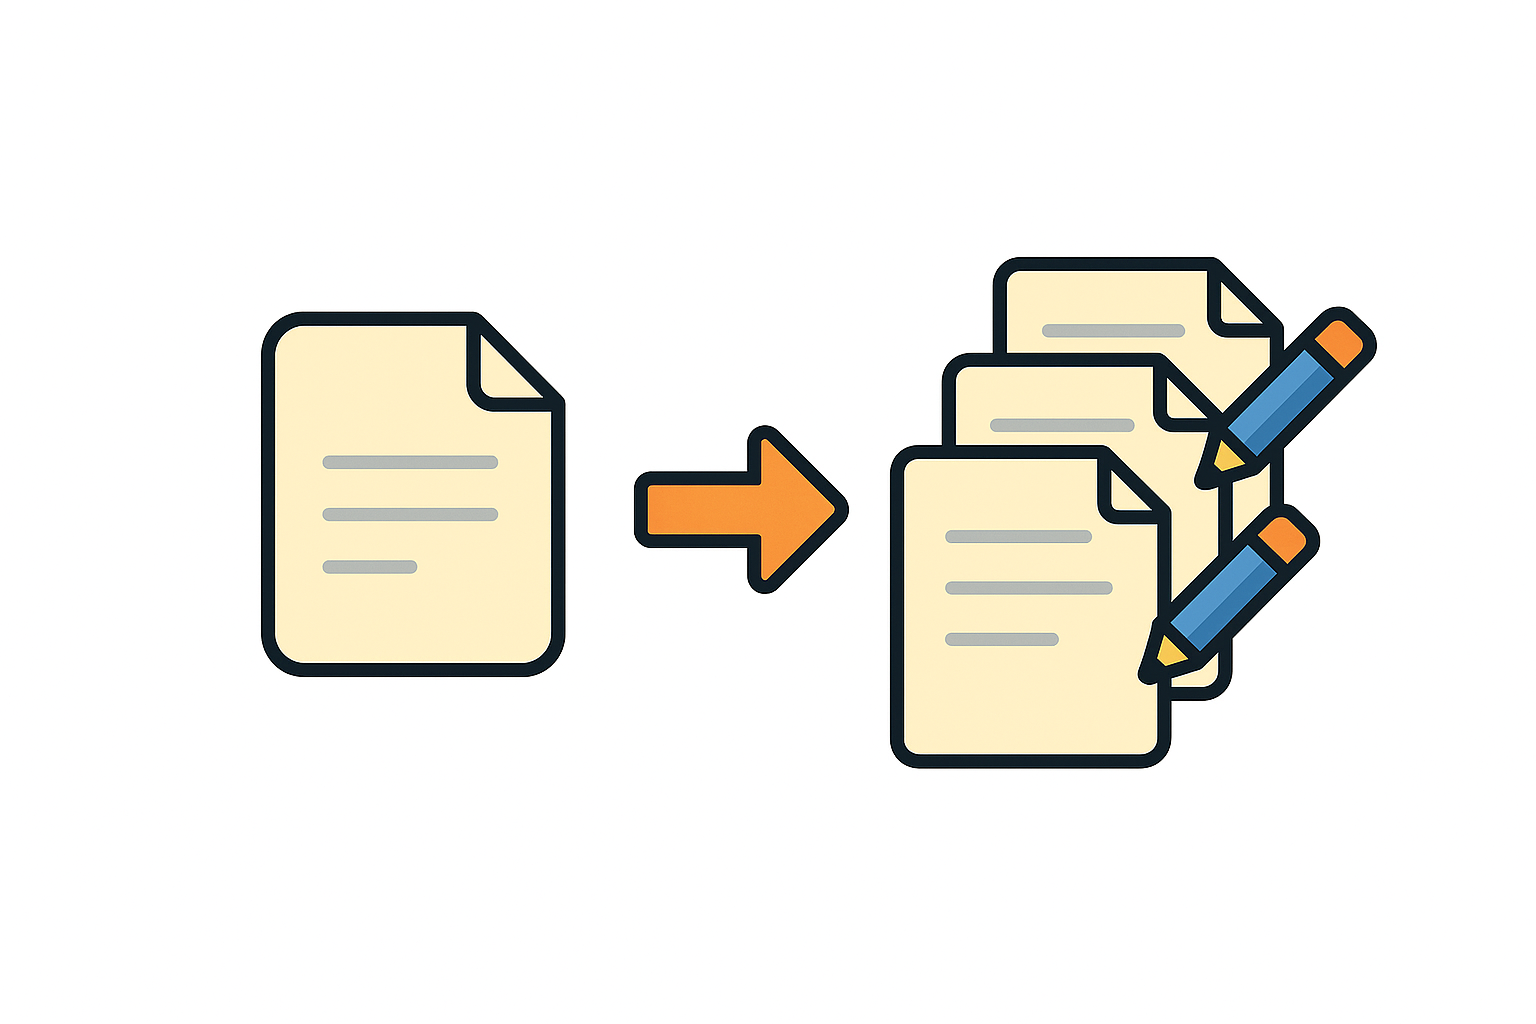
\includegraphics[height=.4\textheight]{figures/FileOperation.png}
    \end{center}

\item Logging into remote server

\item To integrate with other languages and tools.

\item Command Line provides scalability, extensibility, and can automate the entire pipeline for machine learning and data science.


\end{enumerate}
    
\end{frame}

\begin{frame}{Command Line}
    \begin{columns}
        \begin{column}{0.5\textwidth}
            \centering
            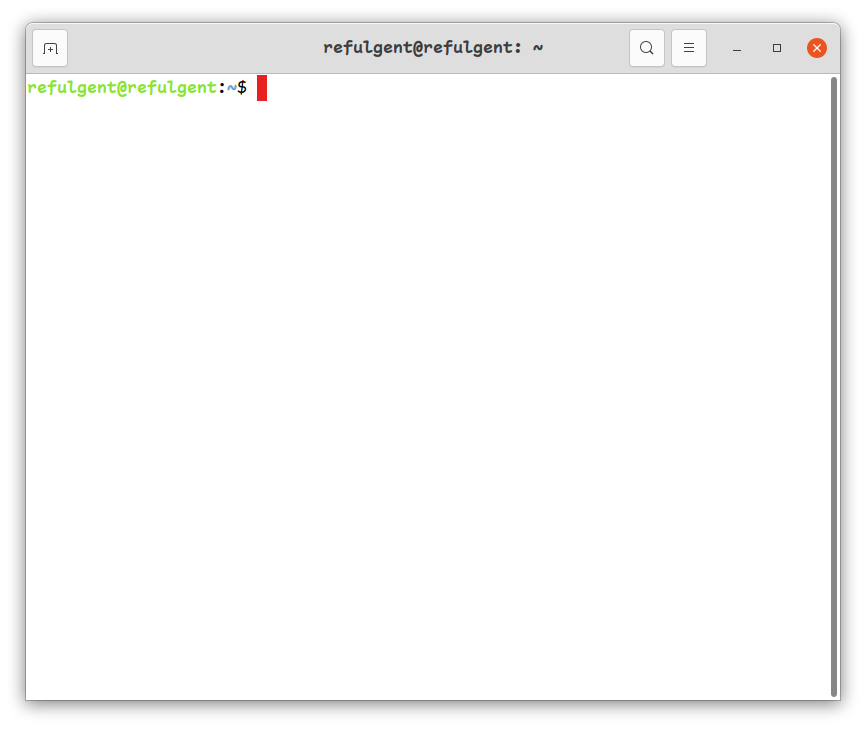
\includegraphics[width=\textwidth,height=1.0\textheight,keepaspectratio]{figures/terminal.png}
        \end{column}
        \begin{column}{0.5\textwidth}
            \begin{enumerate}
                \item Terminals in Linux and Macbook
                \item Windows. Several Options:
                \begin{enumerate}
                    \item Git Bash. Install guide: \url{https://youtu.be/SsdpuprzRE0}
                    \item Cygwin. Install guide: \url{https://youtu.be/_j0Prs7aggo}
                    \item WSL.Install guide: 1. \url{https://youtu.be/GMhV5Uqd8R8},
                    2. \url{https://youtu.be/NPuIUT_6NeM?si=g0N39WfsBf3kIKCx}
                \end{enumerate}
            \end{enumerate}
        \end{column}
    \end{columns}
\end{frame}


\begin{frame}[containsverbatim]{Common Linux Commands}

\footnotesize

My recommendation is to use Windows Subsystem for Linux, as it provides full linux funtionality to Windows.

\vspace{10pt}

A good tutorial to get started is \textbf{Getting started with Linux and Bash
} at \url{https://learn.microsoft.com/en-us/windows/wsl/tutorials/linux}

\begin{tblock}{}

\begin{enumerate}
    \item Installing Software: 
    
    \begin{minted}{bash}
    sudo apt-get install vim git
    \end{minted}

    \item Get the working directory path:
    
    \begin{minted}{bash}
    pwd
    \end{minted}

    \item Change directory:
    
    \begin{minted}{bash}
    cd /data/ch02
    \end{minted}

    \item Create a directory or folder:
    
    \begin{minted}{bash}
    mkdir data
    \end{minted}

\end{enumerate}


\end{tblock}
    
\end{frame}

\begin{frame}
    
    \begin{center}
        An in-depth tutorial is at \url{https://jeroenjanssens.com/dsatcl/chapter-1-introduction}

        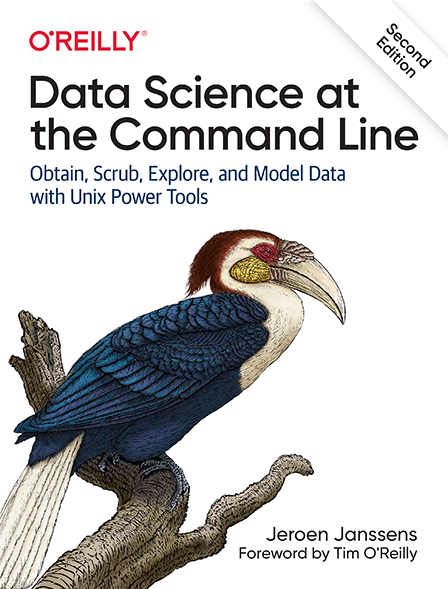
\includegraphics[width=\textwidth,height=0.75\textheight,keepaspectratio]{figures/ds_cmdline.png}

    \end{center}
\end{frame}

\begin{frame}[containsverbatim]{Remote Logging}
    
    If you do not have a powerful machine, you can remotely logging into UAH Engineering Linux Server using your UAH ID.

    \begin{minted}[bgcolor=powderGreen]{bash}
    ssh rkb0022@blackhawk.ece.uah.edu
    \end{minted}

    Windows users should use WSL Terminals.

\end{frame}



\section{Python}

\begin{frame}
    \sectionpage
\end{frame}


\begin{frame}[containsverbatim]{Installing Python}
    
    Most machine learning libraries and codebase are written Python. Python is supported by a strong open-source community.

    Windows users download from \url{https://www.python.org/downloads/}

    Mac users download from \url{https://www.python.org/downloads/macos/}

    Linux users install from command line

    \begin{minted}[bgcolor=powderGreen]{bash}
    sudo apt-get install python3.12
    \end{minted}

    or 

    \begin{minted}[bgcolor=powderGreen]{bash}
    sudo apt-get install python3.12-full
    \end{minted}

    Recommended version of Python for this course is Python 3.12.

\end{frame}

\section{Git and GitHub}

\begin{frame}
    \sectionpage
\end{frame}

\begin{frame}[containsverbatim]{Version Controlling your Development}
    It is must that any of your machine learning project, and in general any coding project should use Git.

    You should already have Git installed in your system through Git, otherwise install.

    \begin{enumerate}
        \item Create a GitHub account and a user name.
        \item Create a new repository.
        \item Clone to local machine:
        
        \begin{minted}[bgcolor=powderGreen]{bash}
        git clone https://github.com/rahulbhadani/TestRepo TestRep
        \end{minted}

    \end{enumerate}
\end{frame}

\begin{frame}[containsverbatim, allowframebreaks]{Commonly used Git Commands}

    \footnotesize

    \begin{enumerate}
        \item Initialize an existing local folder as a git repo.
        \begin{minted}[bgcolor=powderGreen]{bash}
        git init
        \end{minted}
        \item Add remote to your local git folder (Only needs to do once per repo).
        \begin{minted}[bgcolor=powderGreen]{bash}
        git remote add origin https://github.com/rahulbhadani/TestRepo.git
        \end{minted}
        \item Add files for commit.
        \begin{minted}[bgcolor=powderGreen]{bash}
        git add . # add all files
        git add somefile.txt # Add specific file(s)
        \end{minted}
        \item Commit changes with a message before you push to the remote.
        \begin{minted}[bgcolor=powderGreen]{bash}
        git commit -m "Added some files" # add a meaninful message
        \end{minted}
        \item Push to the remote.
        \begin{minted}[bgcolor=powderGreen]{bash}
        git push  # shortcut command
        git push -u origin # push to a specific remote named origin
        git push -u origin2 HEAD:master # push to specific origin's specific branch
        \end{minted}
        \item Pull updates from a remote.
        \begin{minted}[bgcolor=powderGreen]{bash}
        git pull  # shortcut command
        git pull origin master # pull from specific remote
        \end{minted}

        \item Git undo add before commit
        \begin{minted}[bgcolor=powderGreen]{bash}
        git reset filename.txt
        \end{minted}
        \item Git undo add after commit but before push and keep your changes
        \item \begin{minted}[bgcolor=powderGreen]{bash}
        git reset --soft HEAD~1
        \end{minted}
        \item Git undo add after commit but before push and unstage
        \item \begin{minted}[bgcolor=powderGreen]{bash}
        git reset HEAD~1
        \end{minted}
        \item Git undo add after commit but before push and discard every changes
        \item \begin{minted}[bgcolor=powderGreen]{bash}
        git reset --hard HEAD~1 # use n for undoing n multiple commits
        \end{minted}
    \end{enumerate}
    
\end{frame}

\section{Development Environment}

\begin{frame}
    \sectionpage
\end{frame}

\begin{frame}{Integrated Development Environment (IDE)}

    Why use IDEs?
    \begin{enumerate}
        \item Provides integrated view of editor, file explorer, command lines.
        \item Some IDEs provide intellisense for autocomplete.
        \item IDEs are also integrate with compiler/inteprerter -- one click to run your code.
        \item IDEs are beautiful, rich colors and fonts over boring plain text editors.
        \item Many IDEs add support for additional features such as visualization, remote log in, data wranling, etc.
    \end{enumerate}
    
\end{frame}

\begin{frame}{VS Code}
    
    Many IDEs are available such PyCharm, Atom, VS Code.

    \vspace{10pt}

    For this course, I recommend VS Code.

    \begin{center}
        
\includegraphics[width=\textwidth,height=0.45\textheight,keepaspectratio]{figures/vscode.png}
    \end{center}

    VS Code supports several extensions for Python, and other necessary tools.

\end{frame}

\begin{frame}[containsverbatim]{Installing VS Code}

    Download: \url{https://code.visualstudio.com/download}

    On Linux, downloaded deb file can be install at command line:

    \begin{minted}[bgcolor=powderGreen]{bash}
    sudo dpkg -i code_1.103.1-1755017277_amd64.deb
    \end{minted}
    
\end{frame}

\begin{frame}{VS Code Extension}

    Recommended VS Code Extension:
    \footnotesize
    \begin{enumerate}
        \item Jupyter (Microsoft)
        \item Jupyter Notebook Renderers (Microsoft)
        \item Python (Microsoft)
        \item Pylance (Microsoft)
        \item Python Debugger (Microsoft)
        \item Python Environments (Microsoft)
        \item Remote -- SSH (Microsoft)
        \item Remote -- SSH: Editing Configuration Files (Microsoft)
        \item Remote Explorer (Microsoft)
    \end{enumerate}
    
\end{frame}

\begin{frame}{Connecting to Remote Machine in VS Code}

    When connecting to remote machine on VS Code, environment variables of the remote machine takes into effect.

    \vspace{10pt}

    To connect with \texttt{blackhawk.ece.uah.edu} from outside the Engineering building, we need VPN.

    \vspace{10pt}

    Download VPN: \url{https://chargerware.uah.edu/all-software/secure-access-vpn}

    
\end{frame}

\begin{frame}{Connecting to Remote Machine in VS Code}

    \footnotesize
\begin{columns}
    \column{0.5\linewidth}
\begin{center}
    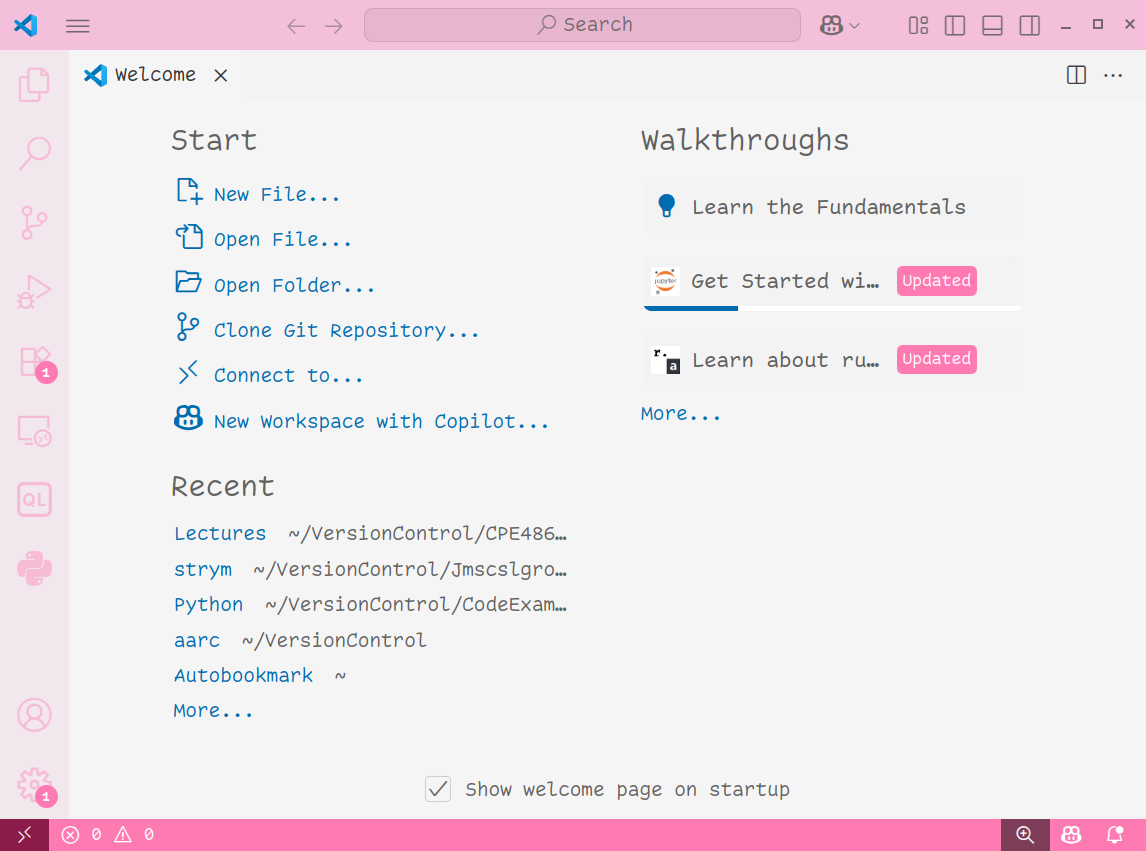
\includegraphics[width=\textwidth,height=0.75\textheight,keepaspectratio]{figures/VSCode_HomePage.png}
\end{center}

    \column{0.5\linewidth}

    After connecting to campus VPN,
    
    click \textbf{Connect to ...}
    
\end{columns}
\end{frame}


\begin{frame}{Connecting to Remote Machine in VS Code}
\footnotesize
\begin{columns}
    \column{0.5\linewidth}
\begin{center}
    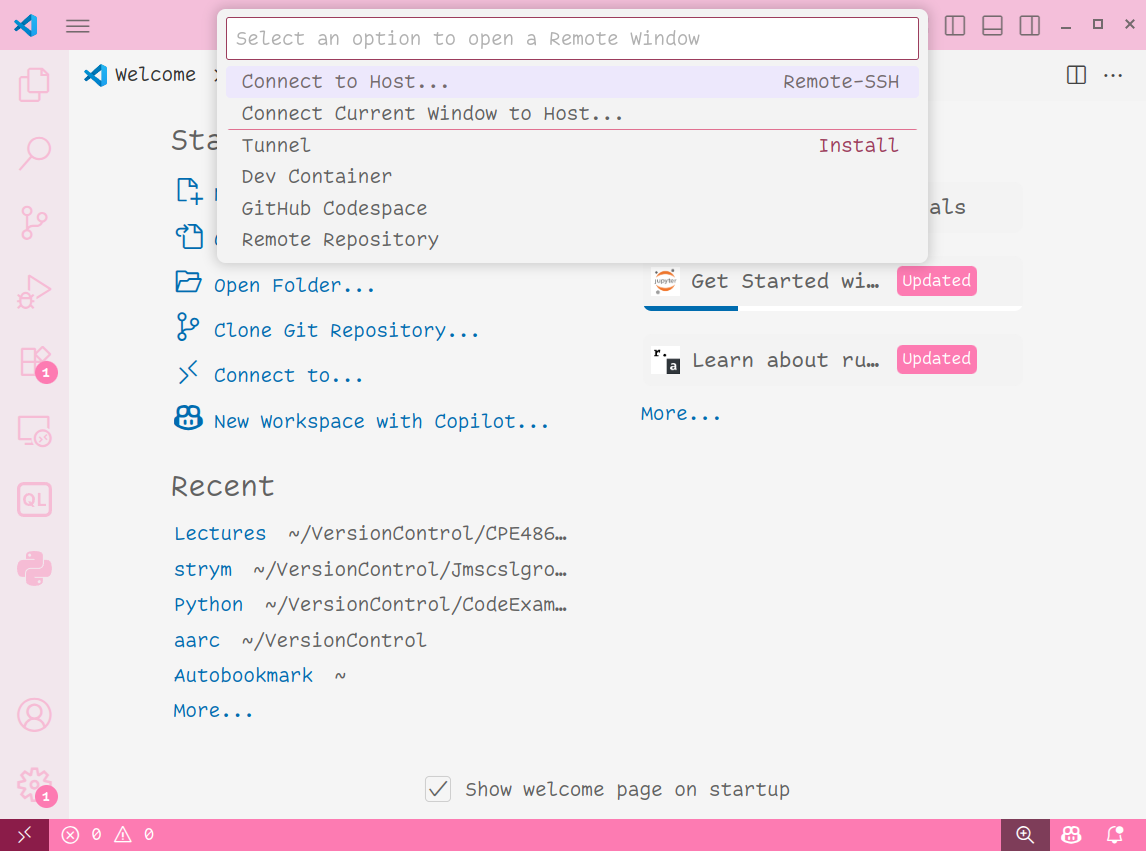
\includegraphics[width=\textwidth,height=0.75\textheight,keepaspectratio]{figures/VSCode_ConnectTo.png}
\end{center}

    \column{0.5\linewidth}

    Click \textbf{Connect to Host ...}, 
    
    enter the address \texttt{username@blackhawk.ece.uah.edu}. Use your own user name.


    
\end{columns}
\end{frame}


\section{Jupyter Notebook}

\begin{frame}
    \sectionpage
\end{frame}


\begin{frame}[containsverbatim]{What is Jupyter Notebook?}
    
    \footnotesize

    Jupyter Notebook is an open source web application which can be used all sorts of data science tasks. The highlight of Jupyter Notebook is reproducibilit and shareability that can combine Markdown, Latex, and plain text for documentation, comments, math, and equations, along with code. In addition, Jupyter also supports Widgets for interactivity, and provides support for multiple programming languages. Some tasks that are possible are:

    \begin{enumerate}
        \item Data cleaning and transformation
        \item Numerical simulation
        \item Exploratory data analysis
        \item Data visualisation
        \item Statistical modeling
        \item Machine learning
        \item Lab notebook
        \item Document sharing
        \item Process documentation
        \item Teaching and learning
    \end{enumerate}

\end{frame}

\begin{frame}{How does Jupyter Notebook Work?}

    \begin{tblock}{}
        It can run locally on your own computer for lightweight use. It can also run on big servers, which we access remotely through the browser, for heavy computation.

    \end{tblock}

    \begin{tikzpicture}[scale=0.5,
    node distance=2.0cm,
    arrow/.style={-{Stealth[length=3mm]}, thick},
    box/.style={rectangle, rounded corners=5pt, minimum width=2cm, minimum height=1cm, text centered, draw=black, thick},
    user/.style={circle, minimum size=1.5cm, draw=black, thick, fill=yellow!80},
    file/.style={rectangle, minimum width=1.5cm, minimum height=2cm, draw=black, thick, fill=gray!20}
]

% Nodes
\node[user] (user) {\Large\Smiley};
\node[box, fill=purple!30, right=of user] (browser) {Browser};
\node[box, fill=green!30, right=of browser] (notebook) {Notebook\\server};
\node[box, fill=green!20, right=of notebook] (kernel) {Kernel};
\node[file, below=1.5cm of notebook] (file) {Notebook file};

% Labels
\node[below=0.2cm of user] {User};

% Arrows
\draw[arrow, <->] (user) -- (browser);
\draw[arrow, <->] (browser) -- node[above, font=\small] {HTTP \&} node[below, font=\small] {Websockets} (notebook);
\draw[arrow, <->] (notebook) -- node[above, font=\small] {ZMQ} (kernel);
\draw[arrow, <->] (notebook) -- (file);

\end{tikzpicture}
    
\end{frame}

\begin{frame}{Jupyter Nootebook}
    

\begin{center}
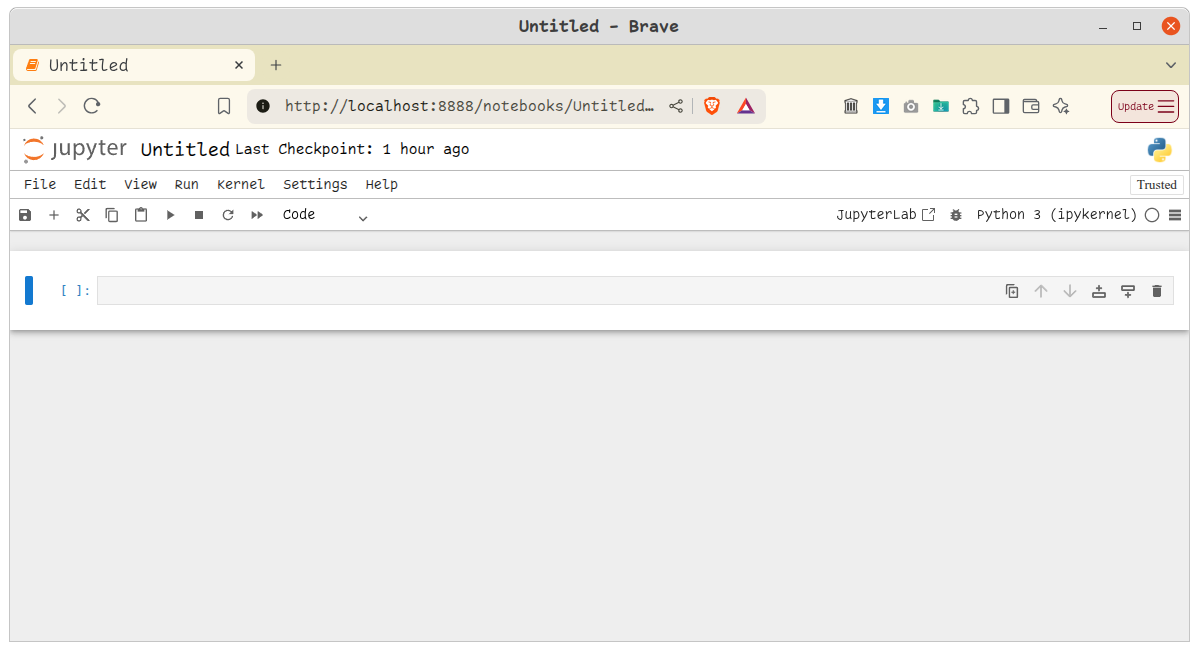
\includegraphics[width=\textwidth,height=0.75\textheight,keepaspectratio]{figures/Jupyter_Screenshot.png}
\end{center}
\end{frame}

\section{Packages and Package Manager}

\begin{frame}
    \sectionpage
\end{frame}


\begin{frame}
    \frametitle{Package / library management – Intro}
    \begin{columns}
        \begin{column}{0.6\textwidth}
            \begin{itemize}
                \item Python has a vast number of packages and libraries
                \item Installation from \textbf{official} Python Package Index
                \begin{itemize}
                    \item Always try to install from the official package manager if possible
                \end{itemize}
                \item The \textbf{pip} tool helps to find and install packages
            \end{itemize}
        \end{column}
        \begin{column}{0.4\textwidth}
            \centering
            
\includegraphics[width=\textwidth]{figures/python_package_index_logo.png}
        \end{column}
    \end{columns}
\end{frame}

\begin{frame}
    \frametitle{Python Packages}
    \begin{itemize}
        \item Python, as a programming language, is rather lean in terms of its built-in functions.
        \item With the help of packages, however, the range of functions can be expanded almost infinitely.
        \begin{itemize}
            \item This is the official third-party software repository for Python.
            \item It's also known as the Cheese Shop (\url{https://youtu.be/Hz1JWzyvv8A}).
        \end{itemize}
    \end{itemize}
    \begin{figure}
        \centering
        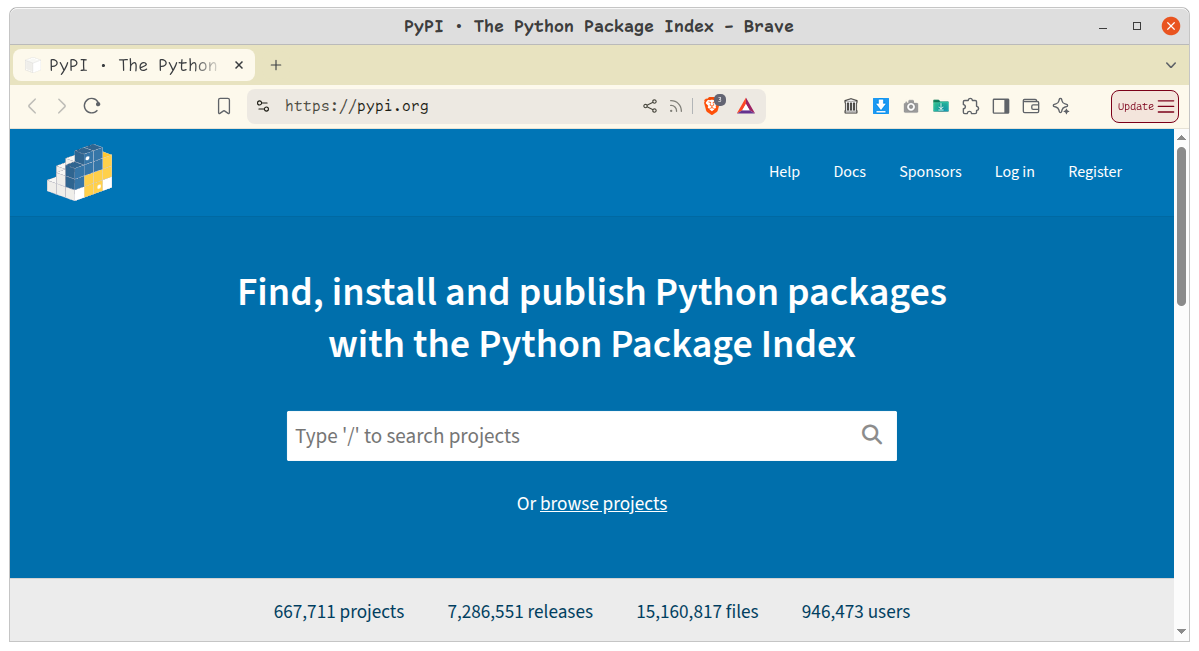
\includegraphics[width=0.4\textwidth]{figures/python_package_index_screenshot.png}
        \caption{A screenshot of the Python Package Index homepage.}
    \end{figure}
\end{frame}

\begin{frame}{Python Package Tool – pip}

    \begin{center}
        Check your versions, you should have v3.0 for both, python \& pip
    \end{center}

    \begin{figure}
        \centering
        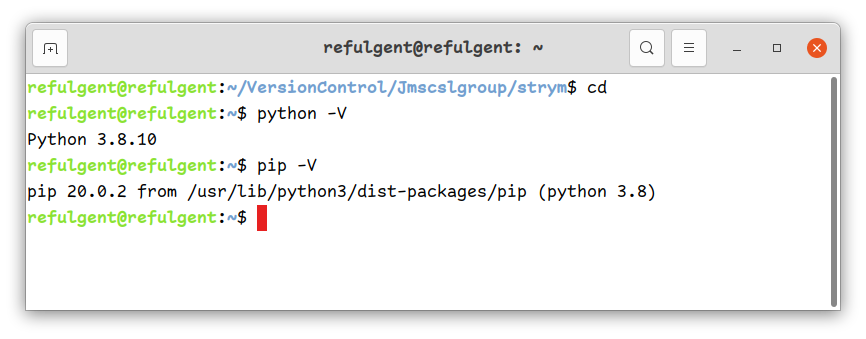
\includegraphics[width=0.6\textwidth]{figures/pipversion.png}
        \caption{Check for PIP version}
    \end{figure}
    
\end{frame}

\begin{frame}[containsverbatim]{Installing Python packages through PIP}

    \begin{minted}[bgcolor=powderGreen]{bash}
pip install numpy # Install specific packages
    \end{minted}

    \begin{minted}[bgcolor=powderGreen]{bash}
pip install -r requirements.txt  # Install packages from a list of files
    \end{minted}
    
\end{frame}

\begin{frame}{Virtual environments}

    \begin{enumerate}
        \item Virtual environments isolate the version of the Python interpreter (Python binary) and all its packages in aseparated directory
        \item Virtual environments are useful when you want to isolate one development activity from another, as some package versions might conflict with another versions.
    \end{enumerate}

    \begin{tikzpicture}[scale=1.0,
    every node/.style={transform shape},
    oval/.style={ellipse, minimum width=3cm, minimum height=2cm, draw, thick, text=white, font=\large},
    site/.style={oval, fill=orange!70, draw=orange!80},
    venv/.style={oval, fill=blue!60, draw=blue!70},
    tag/.style={rectangle, rounded corners=2pt, minimum width=0.6cm, minimum height=0.4cm, 
                text=white, font=\scriptsize\bfseries, draw=white, thick}
]

% Site directory
\node[site] (site) at (0,0) {Site directory};
\node[tag, fill=red!70] at (-0.8, 0.6) {v1};

% Virtual environments
\node[venv] (venv1) at (4, -1.5) {Venv1};
\node[tag, fill=green!60] at (3.2, -1.0) {v2};
\node[tag, fill=blue!80] at (4.8, -1.9) {v1};

\node[venv] (venv2) at (6, 1) {Venv2};
\node[tag, fill=red!70] at (5.0, 1.2) {v1};
\node[tag, fill=blue!80] at (6.0, 0.5) {v3};
\node[tag, fill=green!60] at (6.8, 1.5) {v1};

\node[venv] (venv3) at (8.5, -1) {Venv3};
\node[tag, fill=blue!80] at (7.7, -0.6) {v1};
\node[tag, fill=red!70] at (7.7, -1.4) {v2};

\end{tikzpicture}

    
\end{frame}

\begin{frame}{Introduction to UV}

    % Source: https://uv-introduction-da5541.pages.in2p3.fr/
    \centering
    \huge
    UV is a Python package and project management tool.
    
\end{frame}

\begin{frame}{}

    Once upon a time ... 

    \begin{figure}
        \centering
        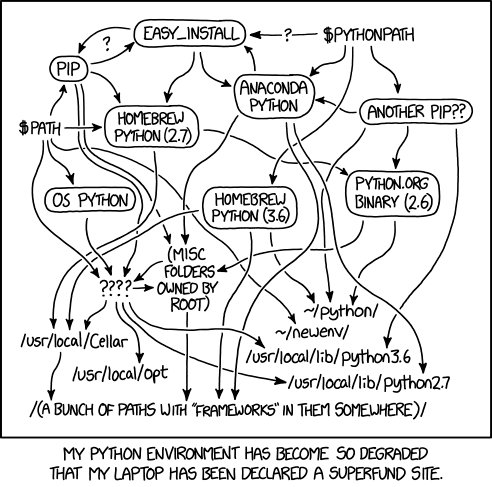
\includegraphics[width=0.4\textwidth]{figures/xkcd.png}
        \caption{\url{https://xkcd.com/1987/}}
    \end{figure}
    
\end{frame}

\begin{frame}
    \frametitle{Objectives}
    \begin{enumerate}
        \item \textbf{Manage packages and dependencies:} \texttt{pip}
        \item \textbf{Each project in its own environment:} \texttt{venv}, \texttt{poetry}, \texttt{hatch}, \texttt{pdm}, \texttt{rye}...
        \item \textbf{Each tool in its own environment:} \texttt{pipx}
        \item \textbf{Manage different Python versions:} \texttt{pyenv}
    \end{enumerate}

    \begin{tblock}{}
        \begin{itemize}
        \item \texttt{uv} can potentially replace them all !!!
    \end{itemize}
    \end{tblock}

\end{frame}

\begin{frame}{Limitation of \texttt{uv}}

    \begin{enumerate}
        \item Not an alternative to Conda.
        \item Can only install Python packages
        \item However, easy to integrate with RUST programming language
    \end{enumerate}
    
\end{frame}


\begin{frame}[containsverbatim]{Installation}

    \begin{enumerate}
        \item Linux/Mac/WSL on Windows:
        \begin{minted}[bgcolor=powderGreen]{bash}
curl -LsSf https://astral.sh/uv/install.sh | sh
\end{minted}

\item Windows:
\begin{minted}[bgcolor=powderGreen,fontsize=\footnotesize]{bash}
powershell -ExecutionPolicy ByPass -c "irm https://astral.sh/uv/install.ps1 | iex"
\end{minted}
\item Doesn't require admin rights
    \end{enumerate}
\end{frame}

\begin{frame}[containsverbatim]{Python version management}

    \begin{enumerate}
        \item \textbf{List installed and available Python versions:}
        \begin{minted}[bgcolor=powderGreen,fontsize=\footnotesize]{bash}
uv python list
        \end{minted}
        \item \textbf{Install a Python version:}
        \begin{minted}[bgcolor=powderGreen,fontsize=\footnotesize]{bash}
# Install latest version
uv python install
        \end{minted}
        \begin{minted}[bgcolor=powderGreen,fontsize=\footnotesize]{bash}
# Install a specific version
uv python install 3.12
uv python install 3.11.10
        \end{minted}
    \end{enumerate}

\end{frame}

\begin{frame}[containsverbatim]{Python version management}

\textbf{Run Python:}
\begin{enumerate}
    \item \textbf{Latest version:}
    \begin{minted}[bgcolor=powderGreen,fontsize=\footnotesize]{bash}
uv run python
\end{minted}
\item \textbf{Specific version:}
\begin{minted}[bgcolor=powderGreen,fontsize=\footnotesize]{bash}
uv run --python 3.11 python
\end{minted}
\item \textbf{System version:}
\begin{minted}[bgcolor=powderGreen,fontsize=\footnotesize]{bash}
python
\end{minted}
\end{enumerate}

\bigskip
\textbf{Note:}
\begin{minted}[bgcolor=lightblue,fontsize=\footnotesize]{text}
uv doesn't modify the PATH.
\end{minted}

\end{frame}

\begin{frame}[containsverbatim]{Python version management}

    \textbf{Pin a Python version in a directory:}
    \begin{minted}[bgcolor=powderGreen,fontsize=\footnotesize]{bash}
# Fix default Python version
cd python_project
uv python pin 3.12
uv run python
    \end{minted}

    \bigskip
    \textbf{If a requested Python version is not installed, \texttt{uv run} will install it automatically:}
    \begin{minted}[bgcolor=powderGreen,fontsize=\footnotesize]{bash}
uv run --python 3.9 python
    \end{minted}

    \bigskip
    \textbf{Remove an installed Python version:}
    \begin{minted}[bgcolor=powderGreen,fontsize=\footnotesize]{bash}
uv python uninstall 3.9
    \end{minted}

\end{frame}

\begin{frame}[containsverbatim]{Dependencies}

    \textbf{Run a Python interpreter with dependencies:}
    \begin{minted}[bgcolor=powderGreen,fontsize=\footnotesize]{bash}
# One dependency
uv run --with numpy python
    \end{minted}
    \begin{minted}[bgcolor=powderGreen,fontsize=\footnotesize]{bash}
# Several dependencies
uv run --with numpy --with matplotlib python
    \end{minted}

    \bigskip
    \textbf{Run a command from a dependency:}
    \begin{minted}[bgcolor=powderGreen,fontsize=\footnotesize]{bash}
# Launch a jupyter lab instance
uv run --with jupyterlab jupyter lab
    \end{minted}
    \begin{minted}[bgcolor=powderGreen,fontsize=\footnotesize]{bash}
# Launch a jupyter lab instance with numpy installed under Python 3.12
uv run --python 3.12 --with jupyterlab --with numpy jupyter lab
    \end{minted}

\end{frame}

\begin{frame}[containsverbatim]{Script dependencies}

    Suppose we have the following \texttt{test.py} script:
    \begin{minted}[bgcolor=powderGreen,fontsize=\footnotesize]{python}
import numpy as np
print(np.random.rand())
    \end{minted}

    We can run the script in a temporary virtual environment with \texttt{numpy} with:
    \begin{minted}[bgcolor=powderGreen,fontsize=\footnotesize]{bash}
uv run --with numpy test.py
    \end{minted}

\end{frame}

\begin{frame}[containsverbatim]{Script dependencies}

    \footnotesize

    We can also add the dependency directly in the script:
    \begin{minted}[bgcolor=powderGreen,fontsize=\footnotesize]{bash}
uv add numpy --script test.py
uv run test.py
    \end{minted}

    Dependencies have been added as inline script metadata (PEP 723):
    \begin{minted}[bgcolor=powderGreen,fontsize=\footnotesize]{python}
# /// script
# requires-python = ">=3.12"
# dependencies = [
#     "numpy",
# ]
# ///
import numpy as np
print(np.random.rand())
    \end{minted}


\begin{center}
    A script with inline metadata can be run with \texttt{uv} on any machine: required python version and dependencies will automatically 
    be installed in a temporary virtual environment.
\end{center}

\end{frame}


\begin{frame}[containsverbatim]{Projects}

    More complex projects must have their own persistent virtual environment.
    \begin{minted}[bgcolor=powderGreen,fontsize=\footnotesize]{bash}
# Create a project in a new folder
uv init my_project
# Create a project in the current folder
uv init .
    \end{minted}

    \bigskip
    \texttt{uv init} will:
    \begin{itemize}
        \item create a \texttt{pyproject.toml} and a \texttt{.python-version} file
        \item initialize a git repository
        \item create sample \texttt{hello.py} and \texttt{README.md} files
    \end{itemize}

\end{frame}

\begin{frame}[containsverbatim]{Projects}

    The \texttt{pyproject.toml} file contains the project metadata and dependencies. It can be edited manually, or via \texttt{uv} commands.

    \begin{minted}[bgcolor=powderGreen,fontsize=\footnotesize]{bash}
# Add a dependency to current project
uv add numpy
# Add a dependency to current project with a minimum version
uv add "polars>=1.6"
# Add a dependency to current project with a specific version
uv add "polars==1.5"

# Remove dependency from current project
uv remove polars

# Add a development dependency
uv add --dev black
    \end{minted}

    \begin{center}
        If your project is itself a Python package, it will be installed in the virtual environment as an editable dependency.
    \end{center}
\end{frame}

\begin{frame}{Projects}

    Dependencies constraints are resolved in the \texttt{uv.lock} lockfile.
    \begin{itemize}
        \item \texttt{uv lock} ensures that the lockfile is still consistent with the dependencies constraints
        \item \texttt{uv sync} synchronizes the virtual environment with the lockfile, installing / removing dependencies if needed
    \end{itemize}

    \begin{block}{Note}
        \begin{itemize}
            \item \texttt{uv lock} and \texttt{uv sync} are automatically run after \texttt{uv add}, \texttt{uv remove} or \texttt{uv run}.
            \item \texttt{uv lock} doesn't upgrade packages if new versions are available. Add \texttt{--upgrade} argument to do it.
        \end{itemize}
    \end{block}

    \begin{block}{Note}
        The virtual environment is created in \texttt{.venv} in the project folder.
        It can still be activated with \texttt{source .venv/bin/activate}.
    \end{block}

\end{frame}

\begin{frame}[containsverbatim]{Projects}

    \texttt{uv run} in a project folder (or one of its subfolders) runs the command inside the project's virtual environment.

    \begin{minted}[bgcolor=powderGreen,fontsize=\footnotesize]{bash}
# Run Python in home folder with no dependencies
cd ~
uv run python
    \end{minted}

    \begin{minted}[bgcolor=powderGreen,fontsize=\footnotesize]{bash}
# Run Python in a project folder. Its dependencies will be available.
cd my_project
uv run python
    \end{minted}

    \begin{minted}[bgcolor=powderGreen,fontsize=\footnotesize]{bash}
# Run a script in the project environment
uv run main.py
    \end{minted}

\end{frame}

\begin{frame}{Projects}

    If an \texttt{uv} project is cloned from a git repository or copied to another machine, running \texttt{uv sync} will install the required Python version and dependencies from its \texttt{uv.lock} lockfile.

    \bigskip
    Running \texttt{uv run} to launch scripts or commands will also automatically lock the dependencies and sync the environment.

\end{frame}

\begin{frame}{Tools}

    Some Python packages are installed for the application they provide:
    \begin{itemize}
        \item \texttt{ruff}
        \item \texttt{black}
        \item \texttt{ipython}
        \item \texttt{py-spy}
        \item \texttt{snakemake}
    \end{itemize}

    \bigskip
    It is highly recommended to install these tools each in their own virtual environment.

\end{frame}

\begin{frame}[containsverbatim]{Tools}

    \texttt{uvx} launches a tool in a temporary environment without installing it:
    \begin{minted}[bgcolor=powderGreen,fontsize=\footnotesize]{bash}
uvx pycowsay "Hello !"
    \end{minted}

    \bigskip
    \texttt{uv tool} allows to install the tool in its own environment and make its binary available in the PATH:
    \begin{minted}[bgcolor=powderGreen,fontsize=\footnotesize]{bash}
uv tool install pycowsay
pycowsay "Hello !"
    \end{minted}

    \begin{talert}{}
    Pay close attention to the package name when running or installing a tool. A wrong name could run a malicious command from a supply chain or typosquatting attack.
    \end{talert}

\end{frame}

\begin{frame}[containsverbatim]{Tools}

    Commands to manage Python tools:
    \begin{minted}[bgcolor=powderGreen,fontsize=\footnotesize]{bash}
# List installed tools
uv tool list

# Install a tool
uv tool install radian

# Upgrade a tool
uv tool upgrade radian
# Upgrade all tools
uv tool upgrade --all

# Uninstall a tool
uv tool uninstall radian
    \end{minted}

\end{frame}

\begin{frame}[containsverbatim]{Tools}

    (Temporary) caveats
    \begin{itemize}
        \item If the default \texttt{uv} Python version is changed, tools need to be reinstalled.
        \item Some tools need workarounds to be installed completely, for example:
    \end{itemize}

    \begin{minted}[bgcolor=powderGreen,fontsize=\footnotesize]{bash}
# To install Snakemake
AR=/usr/bin/ar uv tool install snakemake
    \end{minted}

    \begin{minted}[bgcolor=powderGreen,fontsize=\footnotesize]{bash}
# To install Ansible
uv tool install ansible-core --with ansible
    \end{minted}

\end{frame}


\begin{frame}[containsverbatim]{Creating and Installing a Package with UV}

\begin{minted}[bgcolor=powderGreen,fontsize=\footnotesize]{bash}
# Create a uv project
uv init --lib --package myawesomepackage --build-backend maturin --author-from git
cd myawesomepackage
# install python
uv python install 3.12
# create a virtual environment
uv venv --python 3.12
# activate virtual environment
source .venv/bin/activate
    \end{minted}
    
\end{frame}


\begin{frame}[containsverbatim]{Creating and Installing a Package with UV}

Let's look at the structure of the package:

\begin{Verbatim}[commandchars=\\\{\}]
\textbar{}-- Cargo.toml
\textbar{}-- pyproject.toml
\textbar{}-- README.md
\textbackslash{}\textbar{}-- src
    \textbar{}-- lib.rs
    \textbackslash{}\textbar{}-- myawesomepackage
        \textbar{}-- \_core.pyi
        \textbar{}-- \_\_init\_\_.py
        \textbar{}-- py.typed
\end{Verbatim}

Inside \texttt{src/myawesomepackage} create a folder called \texttt{arithmetic}.

\begin{minted}[bgcolor=powderGreen,fontsize=\footnotesize]{bash}
mkdir arithmetic
cd arithmetic
\end{minted}
\end{frame}

\begin{frame}[containsverbatim]{Creating and Installing a Package with UV}

Now we will create a module in \texttt{arithmetic} subpackage.

\begin{tblock}{Module}
    A module is a file containing Python definitions and statements. A module can contain executable statements as well as function definitions. Read more at \url{https://docs.python.org/3/tutorial/modules.html}
\end{tblock}

\begin{minted}[bgcolor=powderGreen,fontsize=\footnotesize]{bash}
    touch __init__.py # a subpackage must contain __init__.py
    code series.py
\end{minted}

and enter the following code by copying from \url{https://gist.github.com/rahulbhadani/a95e5f57bd7bb906755f443a91d7b0c2}



\end{frame}

\begin{frame}[containsverbatim]{Creating and Installing a Package with UV}

Add the following code to \mintinline{text}|__init__.py|.

\begin{minted}[bgcolor=powderGreen,fontsize=\footnotesize]{bash}
"""
Arithmetic subpackage containing mathematical progression functions.
"""

from .series import arithmetic_progression, arithmetic_sum

__all__ = ['arithmetic_progression', 'arithmetic_sum']

    \end{minted}

\end{frame}

\begin{frame}[containsverbatim]{Creating and Installing a Package with UV}

    \footnotesize

Now, we build the package. Change the directory to the root directory of your \texttt{myawesomepackage}, and type 

\begin{minted}[bgcolor=powderGreen,fontsize=\footnotesize]{bash}
uv build
\end{minted}
    
This will generate a .whl file and a .tar.gz file in \texttt{dist/} folder. You can upload this to GitHub release to be installed later.

Alternatively, you can upload PYPI. You will need to create an account on PYPI and note down your secret code. However, to upload on PYPI, your package need to have a unique name. When you upload on PYPI, you can install from PYPI directly using \mintinline{text}{uv add packagename} or \mintinline{text}{uv pip install packagename}

\begin{minted}[bgcolor=powderGreen,fontsize=\footnotesize]{bash}
uv add twine
twine upload dist/*
\end{minted}

\begin{tblock}{Note:}
    You may need to rename your .whl file so that it ends in \mintinline{text}{...cp39-abi3-manylinux_2_28_x86_64.whl}
    
\end{tblock}


\end{frame}

\begin{frame}[containsverbatim]{Creating and Installing a Package with UV}

    \textbf{Installing the package}

    Let's install package in another UV environment. Open a new terminal, and type

\begin{minted}[bgcolor=powderGreen,fontsize=\tiny]{bash}
uv init arithmetic_test
cd arithmetic_test
uv venv --python 3.12
source .venv/bin/activate
uv add https://github.com/rahulbhadani/CPE486586_FA25/releases/download/0.1/myawesomepackage-0.1.0-cp39-abi3-linux_x86_64.whl
\end{minted}

If you uploaded your package to PYPI, you can install using 

\begin{minted}[bgcolor=powderGreen,fontsize=\footnotesize]{bash}
uv add myawesomepackage 
\end{minted}

or 

\begin{minted}[bgcolor=powderGreen,fontsize=\footnotesize]{bash}
uv pip install myawesomepackage 
\end{minted}
\end{frame}

\begin{frame}[containsverbatim]{Using Installed Package with UV}
    
    We will demonstrate how to use Install Package in UV jusing Jupyter and VS Code. Navigate to the project folder you created and activate the virtual environment:

    \begin{minted}[bgcolor=powderGreen,fontsize=\footnotesize]{bash}
cd arithmetic_test
source .venv/bin/activate
uv add --dev jupyter
uv add --dev ipykernel
# create a kernel for jupyter
uv run ipython kernel install --user --env VIRTUAL_ENV $(pwd)/.venv --name=arithmetic_test

# Launch Jupyter Notebook
jupyter notebook

\end{minted}

It will launch the Jupyter Notebook in your browser. There you can create a new .ipynb file select kernel as \textbf{arithmetic\_test} as it is the name we gave to the kernel above.


    
\end{frame}

\begin{frame}[containsverbatim]{Using Installed Package with UV}

    Now, in the notebook, add the following code and execute

\begin{minted}[bgcolor=powderGreen,fontsize=\footnotesize]{bash}
# Option 1: Import the function directly
from myawesomepackage.arithmetic.series import arithmetic_progression
term_10 = arithmetic_progression(5, 2, 10)
term_10

# Option 2: Import from the subpackage (due to \_\_init\_\_.py)
from myawesomepackage.arithmetic import arithmetic_progression

# Option 3: Import the module
from myawesomepackage.arithmetic import series
result = series.arithmetic_progression(5, 2, 10)
result
\end{minted}

\end{frame}

\begin{frame}{Setting Python Virtual Environment using Anaconda}

    Alternatively, we can use Anaconda instead of UV for virtual environment as well, however, I recommend using UV for this course.

    \begin{center}
        
\includegraphics[width=0.4\linewidth]{figures/Anaconda_Logo.png}\\

        Download: \url{https://www.anaconda.com/download/success}
    \end{center}

\end{frame}

\begin{frame}[containsverbatim]{Creating Virtual Environment in Python using Anaconda}
    \begin{minted}[framesep=1mm, baselinestretch=1.2, fontsize=\normalsize, bgcolor=powderGreen]{python}
    conda create --name pythonenv python=3.11
    conda activate pythonenv
    \end{minted}
\end{frame}

\begin{frame}[containsverbatim]{Installing Jupyter Kernel in Your Anaconda Environment}
    The following code snippet install python kernel for use with Jupyter Notebook within your Anaconda virtual environment.

    \begin{minted}[framesep=1mm, baselinestretch=1.2, fontsize=\normalsize, bgcolor=powderGreen]{python}
    conda install ipykernel
    ipython kernel install --user --name=pythonenv
    conda install jupyter
    jupyter notebook
    \end{minted}
\end{frame}

\begin{frame}{Clound-based Solution}
    \begin{center}
    Google Colab

    \url{https://colab.research.google.com/}
    \begin{itemize}
        \item No local setup needed. 
        \item Packages can be installed as needed.
        \item GPU can be bought if needed.
    \end{itemize}
    \end{center}
\end{frame}


\section{Other Notable Tools}

\begin{frame}
    \sectionpage
\end{frame}


\begin{frame}{Tools helpful for Machine Learning and Data Science}

    \begin{columns}
        \column{0.5\linewidth}
        \begin{enumerate}
            \item R Language and R Studio
            \item Julia Programming Language
            \item Tableau
            \item Power BI
            \item Structured Query Language (SQL)
            \item Statistical Analysis System (SAS)
        \end{enumerate}
    \end{columns}
    
\end{frame}

\begin{frame}
    \Huge{\centerline{\color{bubblegumPink}\textbf{The End}}}
\end{frame}



\end{document}